\documentclass[tikz,border=5pt]{standalone}
\usepackage{pgfplots}
\pgfplotsset{compat=1.18}
\usepackage{amsmath}

\begin{document}
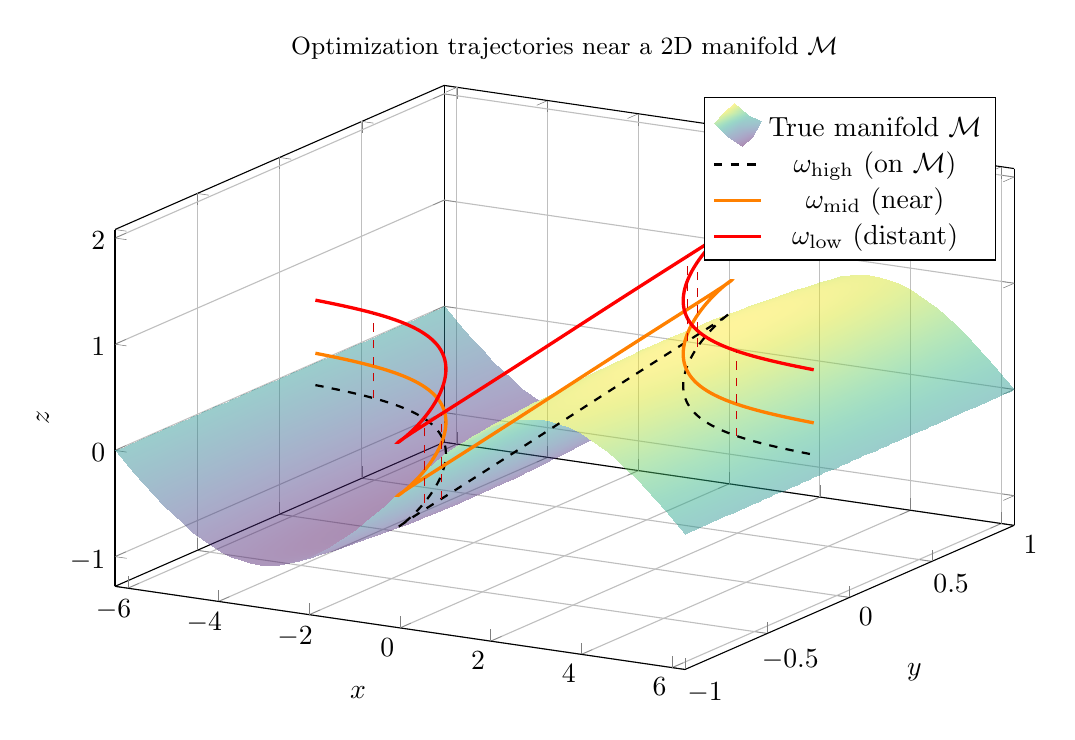
\begin{tikzpicture}
\begin{axis}[
  width=13cm,
  height=9cm,
  view={30}{25},
  xlabel={$x$},
  ylabel={$y$},
  zlabel={$z$},
  domain=-6.283:6.283,
  samples=60,
  y domain=-1:1,
  grid=major,
  colormap/viridis,
  title={Optimization trajectories near a 2D manifold $\mathcal{M}$},
  title style={font=\small},
]

% --- True 2D manifold surface
\addplot3 [surf, opacity=0.45, shader=interp, draw=none]
  {sin(deg(0.5*x))*cos(deg(0.5*y))};

% --- omega values (distance from manifold)
\pgfmathsetmacro{\omegaHigh}{0.0}
\pgfmathsetmacro{\omegaMid}{0.3}
\pgfmathsetmacro{\omegaLow}{0.8}

% === omega_high trajectory (on manifold) ===
\addplot3 [
  domain=-6.0:6.0,
  samples=200,
  samples y=0,
  thick,
  dashed,
  color=black
]
({x},
 {0.5*sin(deg(x))},
 {sin(deg(0.5*x))*cos(deg(0.25*sin(deg(x))))});

% === omega_mid trajectory (near manifold) ===
\addplot3 [
  domain=-6.0:6.0,
  samples=200,
  samples y=0,
  very thick,
  color=orange
]
({x},
 {0.5*sin(deg(x))},
 {sin(deg(0.5*x))*cos(deg(0.25*sin(deg(x)))) + \omegaMid});

% === omega_low trajectory (farther) ===
\addplot3 [
  domain=-6.0:6.0,
  samples=200,
  samples y=0,
  very thick,
  color=red
]
({x},
 {0.5*sin(deg(x))},
 {sin(deg(0.5*x))*cos(deg(0.25*sin(deg(x)))) + \omegaLow});

% === Normal connectors (vertical offsets for illustration)
\foreach \xx in {-5.5,-3.2,-1.1,1.1,3.4,5.3}{
  \pgfmathsetmacro{\yy}{0.5*sin(deg(\xx))}
  \pgfmathsetmacro{\zz}{sin(deg(0.5*\xx))*cos(deg(0.25*sin(deg(\xx))))}
  \addplot3 [orange!80!black, dashed, thin]
    coordinates {(\xx,\yy,\zz) (\xx,\yy,\zz+\omegaMid)};
  \addplot3 [red!80!black, dashed, thin]
    coordinates {(\xx,\yy,\zz) (\xx,\yy,\zz+\omegaLow)};
}

\legend{
  True manifold $\mathcal{M}$,
  $\omega_{\text{high}}$ (on $\mathcal{M}$),
  $\omega_{\text{mid}}$ (near),
  $\omega_{\text{low}}$ (distant)
}

\end{axis}
\end{tikzpicture}
\end{document}

